% One-page layout: (proof-)reading on display
\documentclass[11pt,oneside,a4paper]{book}
% Two-page layout: final printing
%%\documentclass[11pt,twoside,a4paper]{book}   
%=-=-=-=-=-=-=-=-=-=-=-=--=%
% The user of this template may find useful to have an alternative to these 
% officially suggested packages:
\usepackage[czech, english]{babel}
\usepackage[T1]{fontenc} % pouzije EC fonty 
% pripadne pisete-li cesky, pak lze zkusit take:
% \usepackage[OT1]{fontenc} 
\usepackage[utf8]{inputenc}
%=-=-=-=-=-=-=-=-=-=-=-=--=%
% In case of problems with PDF fonts, one may try to uncomment this line:
%\usepackage{lmodern}
%=-=-=-=-=-=-=-=-=-=-=-=--=%
%=-=-=-=-=-=-=-=-=-=-=-=--=%
% Depending on your particular TeX distribution and version of conversion tools 
% (dvips/dvipdf/ps2pdf), some (advanced | desperate) users may prefer to use 
% different settings.
% Please uncomment the following style and use your CSLaTeX (cslatex/pdfcslatex) 
% to process your work. Note however, this file is in UTF-8 and a conversion to 
% your native encoding may be required. Some settings below depend on babel 
% macros and should also be modified. See \selectlanguage \iflanguage.
%\usepackage{czech}  %%%%%\usepackage[T1]{czech} %%%%[IL2] [T1] [OT1]
%=-=-=-=-=-=-=-=-=-=-=-=--=%

%%%%%%%%%%%%%%%%%%%%%%%%%%%%%%%%%%%%%%%
% Styles required in your work follow %
%%%%%%%%%%%%%%%%%%%%%%%%%%%%%%%%%%%%%%%
\usepackage{graphicx}
%\usepackage{indentfirst} %1. odstavec jako v cestine.

\usepackage{k336_thesis_macros} % specialni makra pro formatovani DP a BP
 % muzete si vytvorit i sva vlastni v souboru k336_thesis_macros.sty
 % najdete  radu jednoduchych definic, ktere zde ani nejsou pouzity
 % napriklad: 
 % \newcommand{\bfig}{\begin{figure}\begin{center}}
 % \newcommand{\efig}{\end{center}\end{figure}}
 % umoznuje pouzit prikaz \bfig namisto \begin{figure}\begin{center} atd.

\newcommand\TypeOfWork{Bakalářská práce}  \typeout{Bakalarska prace}
\newcommand\StudProgram{Softwarové technologie a management, Bakalářský}
\newcommand\StudBranch{Softwarové inženýrství}            %pro STM

%%%%%%%%%%%%%%%%%%%%%%%%%%%%%%%%%%%%%%%%%%%%
% Vyplnte nazev prace, autora a vedouciho
% Set up Work Title, Author and Supervisor
%%%%%%%%%%%%%%%%%%%%%%%%%%%%%%%%%%%%%%%%%%%%

\newcommand\WorkTitle{GTD vývojářský úkolovník}
\newcommand\FirstandFamilyName{Ondřej Šatera}
\newcommand\Supervisor{Ing. Macek Ondřej}


% Pouzijete-li pdflatex, tak je prijemne, kdyz bude mit vase prace
% funkcni odkazy i v pdf formatu
\usepackage[
pdftitle={\WorkTitle},
pdfauthor={\FirstandFamilyName},
bookmarks=true,
colorlinks=true,
breaklinks=true,
urlcolor=red,
citecolor=blue,
linkcolor=blue,
unicode=true,
]
{hyperref}



% Extension posted by Petr Dlouhy in order for better sources reference (\cite{} command) especially in Czech.
% April 2010
% See comment over \thebibliography command for details.

\usepackage[square, numbers]{natbib}             % sazba pouzite literatury
%\usepackage{url}
%\DeclareUrlCommand\url{\def\UrlLeft{<}\def\UrlRight{>}\urlstyle{tt}}  %rm/sf/tt
%\renewcommand{\emph}[1]{\textsl{#1}}    % melo by byt kurziva nebo sklonene,
\let\oldUrl\url
\renewcommand\url[1]{<\texttt{\oldUrl{#1}}>}




\begin{document}
\selectlanguage{czech}

% prikaz \typeout vypise vyse uvedena nastaveni v prikazovem okne
% pro pohodlne ladeni prace


\iflanguage{czech}{
	 \typeout{************************************************}
	 \typeout{Zvoleny jazyk: cestina}
	 \typeout{Typ prace: \TypeOfWork}
	 \typeout{Studijni program: \StudProgram}
	 \typeout{Obor: \StudBranch}
	 \typeout{Jmeno: \FirstandFamilyName}
	 \typeout{Nazev prace: \WorkTitle}
	 \typeout{Vedouci prace: \Supervisor}
	 \typeout{***************************************************}
	 \newcommand\Department{Katedra počítačů}
	 \newcommand\Faculty{Fakulta elektrotechnická}
	 \newcommand\University{České vysoké učení technické v Praze}
	 \newcommand\labelSupervisor{Vedoucí práce}
	 \newcommand\labelStudProgram{Studijní program}
	 \newcommand\labelStudBranch{Obor}
}{
	 \typeout{************************************************}
	 \typeout{Language: english}
	 \typeout{Type of Work: \TypeOfWork}
	 \typeout{Study Program: \StudProgram}
	 \typeout{Study Branch: \StudBranch}
	 \typeout{Author: \FirstandFamilyName}
	 \typeout{Title: \WorkTitle}
	 \typeout{Supervisor: \Supervisor}
	 \typeout{***************************************************}
	 \newcommand\Department{Department of Computer Science and Engineering}
	 \newcommand\Faculty{Faculty of Electrical Engineering}
	 \newcommand\University{Czech Technical University in Prague}
	 \newcommand\labelSupervisor{Supervisor}
	 \newcommand\labelStudProgram{Study Programme} 
	 \newcommand\labelStudBranch{Field of Study}
}




%%%%%%%%%%%%%%%%%%%%%%%%%%    Poznamky ke kompletaci prace
% Nasledujici pasaz uzavrenou v {} ve sve praci samozrejme 
% zakomentujte nebo odstrante. 
% Ve vysledne svazane praci bude nahrazena skutecnym 
% oficialnim zadanim vasi prace.
{
\pagenumbering{roman} \cleardoublepage \thispagestyle{empty}
\chapter*{Na tomto místě bude oficiální zadání vaší práce}
\begin{itemize}
\item Toto zadání je podepsané děkanem a vedoucím katedry,
\item musíte si ho vyzvednout na studiijním oddělení Katedry počítačů na Karlově náměstí,
\item v jedné odevzdané práci bude originál tohoto zadání (originál zůstává po obhajobě na katedře),
\item ve druhé bude na stejném místě neověřená kopie tohoto dokumentu (tato se vám vrátí po obhajobě).
\end{itemize}
\newpage
}

%%%%%%%%%%%%%%%%%%%%%%%%%%    Titulni stranka / Title page 

\coverpagestarts

%%%%%%%%%%%%%%%%%%%%%%%%%%%    Podekovani / Acknowledgements 

\acknowledgements
\noindent
Zde můžete napsat své poděkování, pokud chcete a máte komu děkovat.

%%%%%%%%%%%%%%%%%%%%%%%%%%%   Prohlaseni / Declaration 

\declaration{V~Jihlavě dne 29.\,4.\,2012}

%%%%%%%%%%%%%%%%%%%%%%%%%%%%    Abstract 
 
\abstractpage
The purpose of this work is to create tool for developers, which allows them to manage tasks from different services. The tool will be built on a platform of Titanium. An integral part of developing this application will be testing. The aim is to facilitate the application users' work with tasks from different resources / services.

% Prace v cestine musi krome abstraktu v anglictine obsahovat i
% abstrakt v cestine.
\vglue60mm

\noindent{\Huge \textbf{Abstrakt}}
\vskip 2.75\baselineskip

\noindent
Obsahem této práce je vytvoření nástroje pro vývojáře, který umožní správu úkolů z různých služeb. Nástroj bude postavený na platformě Titanium. Nedílnou součástí vývoje bude i testování aplikace. Cílem aplikace je usnadnit uživateli práci s úkoly z různých zdrojů/služeb.

%%%%%%%%%%%%%%%%%%%%%%%%%%%%%%%%  Obsah / Table of Contents 

\tableofcontents


%%%%%%%%%%%%%%%%%%%%%%%%%%%%%%%  Seznam obrazku / List of Figures 

\listoffigures


%%%%%%%%%%%%%%%%%%%%%%%%%%%%%%%  Seznam tabulek / List of Tables

\listoftables


%**************************************************************

\mainbodystarts
% horizontalní mezera mezi dvema odstavci
%\parskip=5pt
%11.12.2008 parskip + tolerance
\normalfont
\parskip=0.2\baselineskip plus 0.2\baselineskip minus 0.1\baselineskip

%**************************************************************

\chapter{Úvod}

Zadáním mojí bakalářské práce je vytvoření nástroje primárně pro vývojáře, kteří pracují na projektech hostovaných na jednom z těchto tří verzovacích serverů: Google Code\cite{gcode}, Assembla\cite{assembla} a GitHub\cite{github}. Nástroj ale poslouží i ostatním vývojářům, byť nejsou primární cílovou skupinou. Využití najde i u neprogramátorů, a to u těch kteří svůj čas organizují metodikou \uv{Getting Things Done}\cite{gtd:web}. Hlavním přínosem mojí práce je usnadnění práce vývojářům, kteří pro správu projektů používají jednu z výše zmíněných služeb. 

Hlavní motivací pro vytvoření této aplikace je snaha usnadnit práci vedoucím týmů, kteří paralelně pracují na více projektech. Tato činnost se může časem stát hodně nepřehlednou protože jsou úkoly roztroušeny na více místech a člověk pak může něco přehlédnout. Aplikace dobře poslouží i samostatným a junior vývojářům. Poskytne jim přehledy dokončených úkolů za aktuální den, týden a měsíc. Zároveň mají možnost nastavit si datum splnění (deadline) úkolů, což ne všechny verzovací servery umožňují. Snadno se tak dozví, kdy už jim dochází čas na splnění konkrétního úkolu. Na světě ale nejsou jen vývojáři, proto je aplikace schopná spravovat i obyčejné projekty, které nejsou nijak svázané s některým z verzovacích systémů. Protože ale tito uživatelé nejsou primární skupinou, pro kterou je aplikace určena, tak na trhu najdou vhodnější nástroje.

Aplikace bude kompletně vytvořena za pomocí vývojového prostředí Titanium Studio\cite{titanium} v rámci platformy \slash frameworku Titanium. Výstupem práce bude kromě samotné aplikace i rešerše této platformy a zhodnocení práce s ní. Jedním z cílů této práce je ověření toho, zda je tato platforma použitelná a zda má smysl se ní nějak hlouběji zabývat.

Mým soukromým cílem a snahou je i to, aby tato aplikace neskončila pouze jako bakalářská práce, ale aby se dále rozvíjela a zlepšovala. Myslím, že má svůj potenciál, a pokud se vyladí hlavně vizuální stránka aplikace, má šanci se uchytit. Proto byl založen web \cite{gtdtoolweb}, kde bude tato práce uveřejněna a kde budou ke stažení veškeré zdrojové kódy včetně dokumentace. Moji ambicí je kolem tohoto projektu vytvořit menší komunitu, která pomůže s dalším rozvojem. V Česku také neexistuje žádný web, který by se věnoval platformě Titanium jako takové, tím jsou moje šance ještě větší.

%*****************************************************************************
%*****************************************************************************
%*****************************************************************************

\chapter{Motivace}

V této kapitole je popsána motivace, kvůli které je tento nástroj vyvíjen. Obsahuje hrubé představení poskytované funkcionality a popis verzovacích serverů, jejichž API je v aplikaci využíváno.

\section{Očekávaná funkcionalita}

Stěžejním úkolem aplikace je správa úkolů a jejich třídění do projektů. Úkoly lze filtrovat podle jim přiřazených štítků a je možné si zvolený výběr vytisknout pro další zpracování. K~úkolům lze přiřadit uživatele, kteří mají na starosti splnění daného úkolu. Zároveň je možné sledovat procentuální splnění jednotlivých projektů pomocí grafů a přehledů.

V tomto nástroji existují v zásadě čtyři typy projektů:

\begin{itemize}
\item obyčejný projekt
\item projekt hostovaný na serveru Assembla
\item projekt hostovaný na serveru Google Code
\item projekt hostovaný na serveru GitHub
\end{itemize}

V další části jsou tyto typy projektů popsány podrobněji.

\subsection{Obyčejný projekt}

Obyčejný projekt neposkytuje žádné speciální funkce, poskytuje pouze možnost roztřídit si úkoly podle nějaké jejich společné vlastnosti. Uživatel si tak může například rozdělit nějaký rozsáhlejší úkol na menší části. Tento projekt ani nemusí souviset s vývojem software.

\subsection{Hostované projekty}

Projekty, které jsou uloženy na některém ze serverů. Tyto jsou vždy pevně svázány s některým z repozitářů, uložených na daném serveru. Poskytují tak možnost synchronizace úkolů, uložených na serveru, s těmi v aplikaci. Při synchronizaci se zároveň stáhne seznam uživatelů, milníků a štítků, které je pak možné dále využívat. Například je možné do milníku přiřadit nový úkol a změna se automaticky projeví i na serveru. To samé je možné při přiřazování úkolů uživatelům.

\subsubsection{Porovnání verzovacích serverů}

Každý ze serverů poskytuje jiné funkce, tzn. že i API jednotlivých služeb budou jiná. To přináší komplikace při vývoji nástroje, který má v sobě integrovat správu všech tří služeb.

Každé z trojice používaných API poskytuje jiný přístup k datům uloženým na serveru. Assembla a Google Code se spoléhá na rozhraní typu REST\cite{rest}. Github používá pro přenos dat JSON\cite{json} pole, která jsou snadněji zpracovatelná JavaScriptem a pomalu se dostávají i do jiných programovacích jazyků. Nejlépe zdokumentované rozhraní má jednoznačně Github. V dokumentaci lze najít i chybové hlášky a všechny typy návratových polí. Github zároveň poskytuje největší paletu nabízených služeb a klientská aplikace se tak dostane kamkoliv. Samotná webová aplikace Githubu běží nad tímto API.

Nejhůře je na tom s dokumentací Assembla, kde polovina údajů chybí a postup práce s~API je tak spíše pokus-omyl. Nikde například nejsou k nalezení chybové hlášky, které API vrací, pokud požadavek z nějakého důvodu nevyhovuje. Vývojáři tak nezbývá nic jiného, než odpověď hledat pomocí vyhledávače.

Google Code má dokumentaci obstojnou, i když pod úrovní dokumentace na Githubu. Některé informace jsou zapsány poměrně nelogicky a v místech, kde by je člověk nehledal. Svůj účel ale dokumentace plní a na většinu otázek dokáže odpovědět.

Služby jsou rozdílné i z jiného úhlu pohledu - z pohledu uživatele. Pro lepší přehlednost jsou tyto rozdíly uvedeny v následující tabulce \ref{tab:versionSystemsDifference}:

\begin{table}
\begin{center}
	\begin{tabular}{|c||l|l|l|}
	\hline
	Funkce & Assembla & GitHub & Google Code \\
	\hline
	\hline
	Definování milníku & ano & ano & ano \\
	Přiřazení štítků k issue & ne & ano & ano \\
	Více různých stavů issue & ano & ne & ano \\
	Nastavení priority & ano & ne & ano \\
	Uložení aktivity u issue & ano & ne & ne \\
	Přidání přílohy k issue & ano & ne & ano \\
	Sledování aktivity v issues & ano & ne & ano \\
	\hline
	Cena za měsíc & od 9 (1GB) & od 7 (0,6GB) & - \\
	(pro komerční projekty) & do 99 dolarů (20GB) & do 22 dolarů (2,4GB) & \\
	\hline
	\end{tabular}
\end{center}
\caption{Rozdíly mezi verzovacími servery}
\label{tab:versionSystemsDifference}
\end{table}

Kvůli těmto rozdílům jsou nutné různé kompromisy, aby bylo možné aplikaci používat konzistentně bez ohledu na to, kde je projekt hostován. Ukazuje se, že GitHub má sice nejlepší dokumentaci, ale ve funkcionalitě pokulhává. Assembla, jejíž dokumentace je nejhorší, naopak poskytuje mnoho funkcí navíc. Assembla je však více zaměřená na komerční projekty, kdežto zbylé dvě služby jsou orientovány spíše na open-source vývojáře. Google Code neumožňuje hostovat komerční projekty vůbec. GitHub má i placený hosting projektů, ale jeho možnosti jsou mnohem menší než u konkurenční Assembly.

\subsection{Getting Things Done}

Tato metoda byla vytvořena americkým koučem Davidem Allenem, který ji popsal ve stejnojmenné knize \cite{gtd:book}. Neslouží přímo k organizaci času, ale orientuje se spíše na organizaci práce a její plánování. Hlavní myšlenkou Allenovy práce je fakt, že lidský mozek není diář a není uzpůsoben k tomu, aby si pamatoval každý úkol a závazek, který je nutno splnit. Člověk pracuje lépe, pokud se nemusí zatěžovat přemýšlením, co všechno musí udělat. Jádrem této metody jsou proto různé seznamy zahrnující úkoly, které je nutno vyřešit. Mozek se tak může soustředit čistě na práci a není rozptylován vzpomínáním na jiné nesouvisející úkoly.

Celou metodu lze rozdělit do pěti kroků\cite{gtd:wiki}:

\begin{itemize}
\item sběr úkolů
\item zpracování
\item zorganizování
\item zhodnocení
\item vykonání
\end{itemize}

V aplikaci jsou zachyceny pouze prostřední tři kroky. Sběr úkolů je nutné provádět průběžně, tzn. nemusí to být v dosahu počítače. Tomuto účelu bohatě postačí papírový zápisník, příp. poznámky uložené v telefonu. Poslední krok \uv{vykonání} je zase plně v režii člověka, tam už žádná aplikace nepomůže.

V kroku \uv{zpracování} dochází k přesunu úkolů z různých zdrojů (zápisník, poznámky) do jedné schránky - aplikace. Nesplnitelné úkoly se buď zahodí nebo se uloží na později. Splnitelné úkoly se buď vykonají, přiřadí někomu jinému nebo uloží na později. O tom, zda se úkol vykoná hned nebo uloží, rozhoduje pravidlo 2 minut. Pokud vykonání úkolu zabere víc času než tyto dvě minuty, je uložen k pozdějšímu zpracování. Zároveň pokud je krok komplexnější a k jeho splnění je potřeba víc než jeden krok, je tento rozdělen na víc částí a uložen jako projekt.

V další fázi - zorganizování - dochází k rozdělení úkolů do těchto pěti oblastí:

\begin{itemize}
\item další kroky - realizovatelné, fyzicky viditelné činnosti, které vedou k nějakému výsledku
\item delegované úkoly - přiřazené jiným lidem, u kterých čekáme na zpracování
\item projektové úkoly
\item úkoly uložené na později
\item naplánované úkoly - mají pevně dané datum splnění (deadline)
\end{itemize}

Čtvrtá fáze, která je zde označena jako zhodnocení, probíhá paralelně se všemi ostatními. Během ní člověk přehodnocuje, zda dělá to, co by dělat měl. K tomu mu poslouží seznam nesplněných úkolů a projektů. Ke zhodnocení dochází také jednou za týden, kdy se upravuje seznam úkolů tak, aby byl aktuální.

\section{Důvody zvolení desktopové aplikace}

V dnešní době už desktopové aplikace vycházejí z módy. Všechna data a aplikace se přesouvají do webového prostoru, kde je obsah přístupný odkudkoliv a je jedno, přes jaké zařízení se k~němu přistupuje. Dokumenty tak lze vytvářet na stolním počítači a pak je upravovat je na~svém smartphonu, který má připojení k internetu. Používání webových úložišť má ale i svá úskalí - bezpečnost a spolehlivost.

\subsection{Bezpečnost}

Data na internetu jsou uložena na vzdáleném serveru a není jisté, že k nim nemá přístup někdo nepovolaný. U desktopových aplikací lze bezpečnost snadno zajistit minimálně pomocí hesla, příp. šifrováním obsahu na pevném disku. Záleží tedy na uživateli, zda se spolehne na~zabezpečení vzdáleného serveru nebo bude mít raději vše pod přímou kontrolou na vlastním počítači. Dalším faktorem, který může rozhodování ovlivnit, je zálohování dat. Pokud je obsah uložen na jednom pevném disku, zvyšuje se pravděpodobnost ztráty dat, takže je nutné pravidelné zálohování. U vzdálených serverů je obvykle o zálohování postaráno automaticky. 

Jak vidno, obě varianty mají svá pro i proti. Důvody pro zvolení desktopové aplikace jsou v zásadě dva - rešerše práce s vývojovým prostředím Titanium Studio a experiment, zda je možné napsat kompletní aplikaci pouze pomocí JavaScriptu. 

\subsection{Využití JavaScriptu}

JavaScript se v poslední době opět vrací na výsluní a lze jej nalézt téměř na každé webové stránce či webové aplikaci. Na rozdíl od ostatních technologií, jako je Flash \cite{flash} nebo Silverlight \cite{silverlight}, není závislý na platformě a funguje stejně dobře na operačním systému Windows, Linux nebo Mac. Jeho podpora je pevně zabudována do drtivé většiny webových prohlížečů a v poslední době se jeho podpora rozšiřuje i na mobilní zařízení. Žádná jiná technologie nemá takovou podporu. JavaScript je nejsnadnější způsob, jak udělat stránku interaktivní. Změnit to může snad jedině větší rozšíření HTML 5, ale to bude ještě nějakou dobu trvat.

%*****************************************************************************
%*****************************************************************************
%*****************************************************************************

\chapter{Analýza}

Pro vývoj aplikace v této bakalářské práci byla zvolena novější - agilní - metodika vývoje, která je v mnoha ohledech jednodušší než dříve používaný Rational Unified Process (RUP)\cite{rup}. Hlavní výhoda spočívá v tom, že se nevytváří hromady dokumentů, jejichž vytvoření zabere spoustu času a ve finále je většina z nich zbytečná. RUP má smysl spíše u velkých projektů, na kterých pracuje větší tým lidí a které jsou hodně rozsáhlé. 

RUP a agilní metodiky se liší už ve způsobu sběru požadavků. Zatímco RUP je orientovaný na use-case modely, vytvářené obvykle v jazyce Unified Modeling Language (UML)\cite{uml}, agilní metodiky evidují požadavky v podobě tzv. user stories \cite{userstory}.

\section{User stories}

Požadavky v rámci agilních metodik se nezapisují jako prosté úkoly, ale mají formát tzv. user story. Jejich tvar je pevně daný a skládá se ze tří částí:
\begin{quote}
Jako \textbf{Uživatel}, chci \textbf{Funkcionalitu} abych dostal \textbf{Bussiness Value}
\end{quote}

Takto formulovaný požadavek je pro člověka mnohem srozumitelnější, protože vidí proč daný úkol splnit a jaký je jeho přínos. Má tak jistotu, že nedělá něco zbytečného. User story je takový krátký příbeh a jako takový je lidským mozkem snáz vnímatelný.

User stories poslouží i po ukončení vývoje - při akceptačních testech. Stačí projít seznam user stories a pokud je v aplikace nalezen jejich \uv{odraz}, test byl úspěšný. Proto je lepší, aby user stories prošly schválením od zadavatele ještě před začátkem vývoje aplikace.

V rámci této bakalářské práce byl vytvořen následující seznam user stories, který je pro lepší přehlednost rozdělen do bloků podle cílové skupiny. Každý blok je uveden názvem role, kde lomítko značí \uv{dědičnost}. Jsou v něm zachyceny všechny požadavky, které by měla aplikace po ukončení vývoje splňovat.

\subsection{Uživatel}

Jako uživatel chci:

\begin{itemize}
\item používat aplikaci co nejjednodušeji, abych se mohl plně soustředit na přesné zadání úkolu
\item vytvářet úkoly, abych na nic nezapomněl
\item vytvářet projekty, abych si mohl úkoly třídit
\item vkládat okažité nápady do inboxu s tím, že je později zatřídím do projektu
\item označit úkol jako splněný
\item uložit úkol do archivu, kdybych se k němu chtěl někdy později vrátit
\item vyhodit úkol do koše, pokud se rozhodnu, že ho nebudu realizovat
\item přidávat úkolům štítky, abych si mohl odfiltrovat úkoly z určité oblasti
\item na konci týdne vědět, co všechno jsem za týden stihl, abych si mohl lépe naplánovat úkoly na příští týden
\item své nápady, na které teď nemám čas, přiřadit do skupiny s delším časovým horizontem, abych na ně nezapomněl a mohl je později rozvíjet
\item vytisknout svoje úkoly, abych je mohl mít neustále na očích
\end{itemize}

\subsection{Uživatel \slash  vývojář}

Jako vývojář chci:

\begin{itemize}
\item importovat projekty a úkoly z verzovacích serverů
\item být informován o blížící se deadline úkolů
\item aby aplikace neumožňovala přístup neoprávněným osobám k mým úkolům
\item spárovat úkol s konkrétním commitem do repozitáře
\item exportovat úkol a poslat ho jednoduše kolegovi v týmu, aby ho nemusel ručně přepisovat
\end{itemize}

\subsection{Uživatel \slash  vývojář \slash  senior}

Jako senior vývojář chci: 

\begin{itemize}
\item párovat repozitáře z verzovacích serverů s mými projekty, abych mohl sledovat, jak práce na projektu pokračuje
\item párovat issues ze serveru s mými úkoly, abych s nimi mohl párovat commity
\item nastavit úkolům čas, kdy mají být splněny
\item delegovat úkoly junior vývojářům
\item přiřadit úkol do konkrétního milníku, abych měl přehled o tom, kolik toho ještě zbývá dokončit
\item být informován o změnách v mých repozitářích na serverech
\item uzavřít projekt, po jeho dokončení příp. předčasném ukončení
\item přidávat štítky k úkolům, abych je mohl lépe třídit a filtrovat
\item být upozorněn na neaktivní otevřené projekty, abych mohl urgovat dokončení úkolů na junior vývojářích
\item mazat úkoly, které se nakonec realizovat nebudou
\item zpřesňovat zadání úkolů, pokud dojde k nejasnostem
\end{itemize}

\subsection{Uživatel \slash  vývojář \slash  junior}

Jako junior vývojář chci:

\begin{itemize}
\item být informován o nově přiřazených úkolech od senior vývojářů
\item označit úkol jako splněný
\end{itemize}

\section{Doménový model}
Z výše zmíněných user stories byl v dalším kroku vytvořen seznam entit, které byly logicky provázány asociacemi. Pro lepší znázornění těchto entit a vztahů mezi nimi byl vytvořen doménové model v jazyce UML.

\begin{figure}[h]
	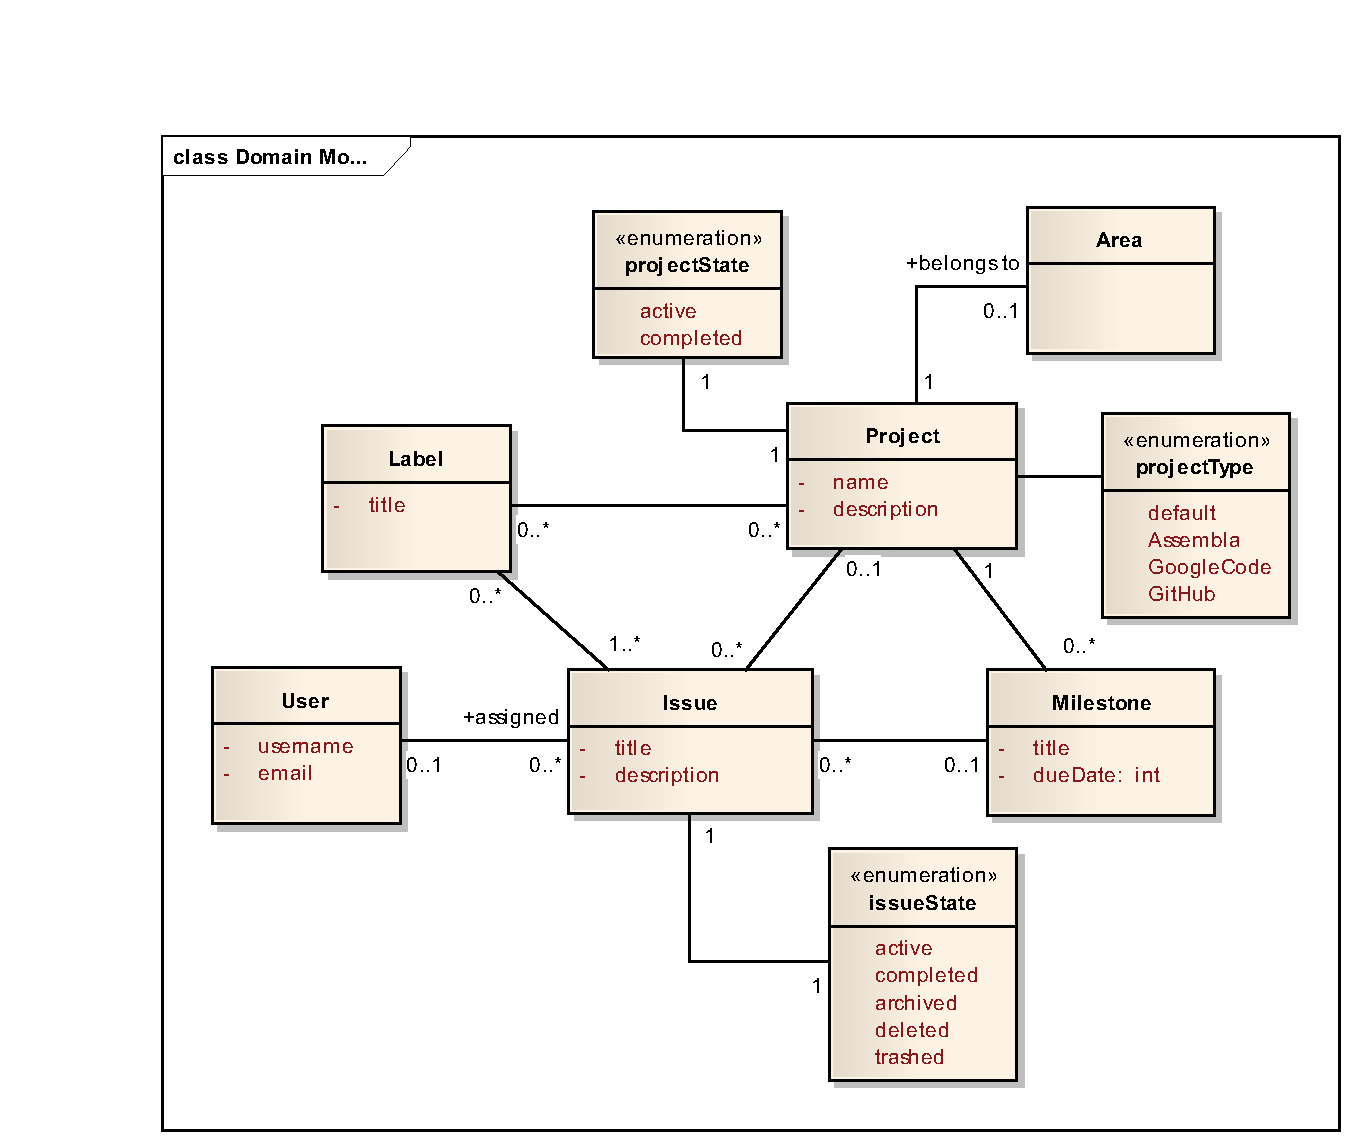
\includegraphics[keepaspectratio,width=16cm]{figures/domain-model}
	\caption{Doménový model}
	\label{fig:domain-model}
\end{figure}

\subsection{Issue}
Entita reprezentující jeden úkol, uložený v aplikaci. Má definované jméno (název problému) a popis, který obsahuje konkrétní popis problému

\subsection{IssueState}
Úkoly (issues) existují v aplikaci v různých stavech. Každý stav určuje jak bude aplikace s daným úkolem zacházet \ref{tab:issueState}.

\begin{table}[h]
\begin{center}
	\begin{tabular}{|c|l|}
	\hline
	Atributy & Poznámky \\
	\hline
	active & na úkolu se pracuje \\
	completed & úkol byl splněn \\
	archived & úkol byl uložen do archivu \\
	deleted & úkol byl smazán \\
	trashed & úkol byl přesunout do koše \\
	\hline
	\end{tabular}
\end{center}
\caption{Vlastnosti entity IssueState}
\label{tab:issueState}
\end{table}

\subsection{Label}
Štítky (label) slouží k filtraci úkolů (issues) a projektů (projects). Obvykle popisují nějakou obecnější vlastnost dané entity, podle které má smysl je filtrovat. To může být například priorita, programovací jazyk nebo náročnost \ref{tab:label}.

\begin{table}[h]
\begin{center}
	\begin{tabular}{|c|l|}
	\hline
	Atributy & Poznámky \\
	\hline
	title & text štítku \\
	\hline
	\end{tabular}
\end{center}
\caption{Vlastnosti entity Label}
\label{tab:label}
\end{table}

\subsection{Milestone}
Milestone se do češtiny překládá jako milník. Je to nějaký bod v čase, do kterého musí být dokončená určitá množina úkolů (issues). Lze sledovat procentuální dokončení \ref{tab:milestone}.

\begin{table}[h]
\begin{center}
	\begin{tabular}{|c|l|}
	\hline
	Atributy & Poznámky \\
	\hline
	title & název milníku \\
	dueDate & do kdy musí být milník splněn \\
	\hline
	\end{tabular}
\end{center}
\caption{Vlastnosti entity Milestone}
\label{tab:milestone}
\end{table}

\subsection{User}
Uživatel (User) vystupuje v aplikaci jako člen týmu, kterému je možné přiřadit nějaký úkol (Issue) \ref{tab:user}.

\begin{table}[h]
\begin{center}
	\begin{tabular}{|c|l|}
	\hline
	Atributy & Poznámky \\
	\hline
	username & uživatelské jméno \\
	email & e-mailová adresa uživatele \\
	\hline
	\end{tabular}
\end{center}
\caption{Vlastnosti entity User}
\label{tab:user}
\end{table}

\subsection{Project}
Úkoly (issues) jsou uspořádané do projektů, které mají definované jméno a popis. I z úkolu se může stát projekt pokud je k jeho dokončení potřeba víc než jeden krok (podle GTD) \ref{tab:project}.

\begin{table}[h]
\begin{center}
	\begin{tabular}{|c|l|}
	\hline
	Atributy & Poznámky \\
	\hline
	name & název projektu \\
	description & popis projektu \\
	\hline
	\end{tabular}
\end{center}
\caption{Vlastnosti entity Project}
\label{tab:project}
\end{table}

\subsection{ProjectState}
Projekt může být buď aktivní, tzn. že se na něm pracuje, nebo dokončený \ref{tab:projectState}.

\begin{table}[h]
\begin{center}
	\begin{tabular}{|c|l|}
	\hline
	Atributy & Poznámky \\
	\hline
	active & aktivní \\
	completed & dokončený \\
	\hline
	\end{tabular}
\end{center}
\caption{Vlastnosti entity ProjectState}
\label{tab:projectState}
\end{table}

\subsection{ProjectType}

Každý projekt má definovaný nějaký typ, podle kterého se určí na jaký server se má synchronizovat. Pokud jde o obyčejný projekt (default) nesynchronizuje se nikam, všechny úkoly zůstávají pouze na lokálním úložišti \ref{tab:projectType}.

\begin{table}[h]
\begin{center}
	\begin{tabular}{|c|l|}
	\hline
	Atributy & Poznámky \\
	\hline
	default & obyčejný GTD projekt \\
	Assembla & projekt hostovaný na serveru Assembla.com \\
	GoogleCode & projekt hostovaný na serveru Google Code \\
	GitHub & projekt hostovaný na serveru GitHub.com \\
	\hline
	\end{tabular}
\end{center}
\caption{Vlastnosti entity ProjectType}
\label{tab:projectType}
\end{table}

\subsection{Area}

Projekty (project) lze zařadit do nějaké oblasti (area), což může být např. škola, práce, vzdělávání apod. Cílem je zpřehlednění seznamu projektů.

%*****************************************************************************
%*****************************************************************************
%*****************************************************************************

\chapter{Architektura}

Návrh architektury této aplikace byl výrazně ovlivněn dvěma fakty. Za prvé jde o aplikaci vyvíjenou kompletně v JavaScriptu, který není objektovým ale spíš skriptovacím programovacím jazykem a některé konstrukce nejsou možné (např. rozhraní, abstraktní třídy apod.). Nemalý vliv měla i samotná platforma Titanium, která je do aplikace pevně zadrátována a která si vyžádala určité kompromisy, ale zároveň umožnila zjednodušení celé aplikace.

\section{Rozdělení do balíčků}

Aplikaci lze rozdělit do několika balíčků, i když toto rozdělení není tak patrné jako například u Javy. Jako vzor pro celkovou architekturu bylo zvoleno MVC (model-view-controller), kde je oddělená prezentační část od výkonné a obsahové. Nicméně to vyžadovalo pár kompromisů protože JavaScript není primárně objektový jazyk.

Celá aplikace využívá ke svému běhu knihovnu PrototypeJS\cite{prototypejs}, díky které lze snadno definovat objekty a omezeně i dědičnost mezi nimi. V prezentační části se navíc využívá knihovna Script.aculo.us\cite{scriptaculous}, která je postavena na dříve zmíněném PrototypeJS a která umožňuje snadnější vytváření efektů a různých animací.

Diagram \ref{fig:class-model} znázorňuje rozdělení aplikace do balíčků.

\begin{figure}[h]
\begin{center}
	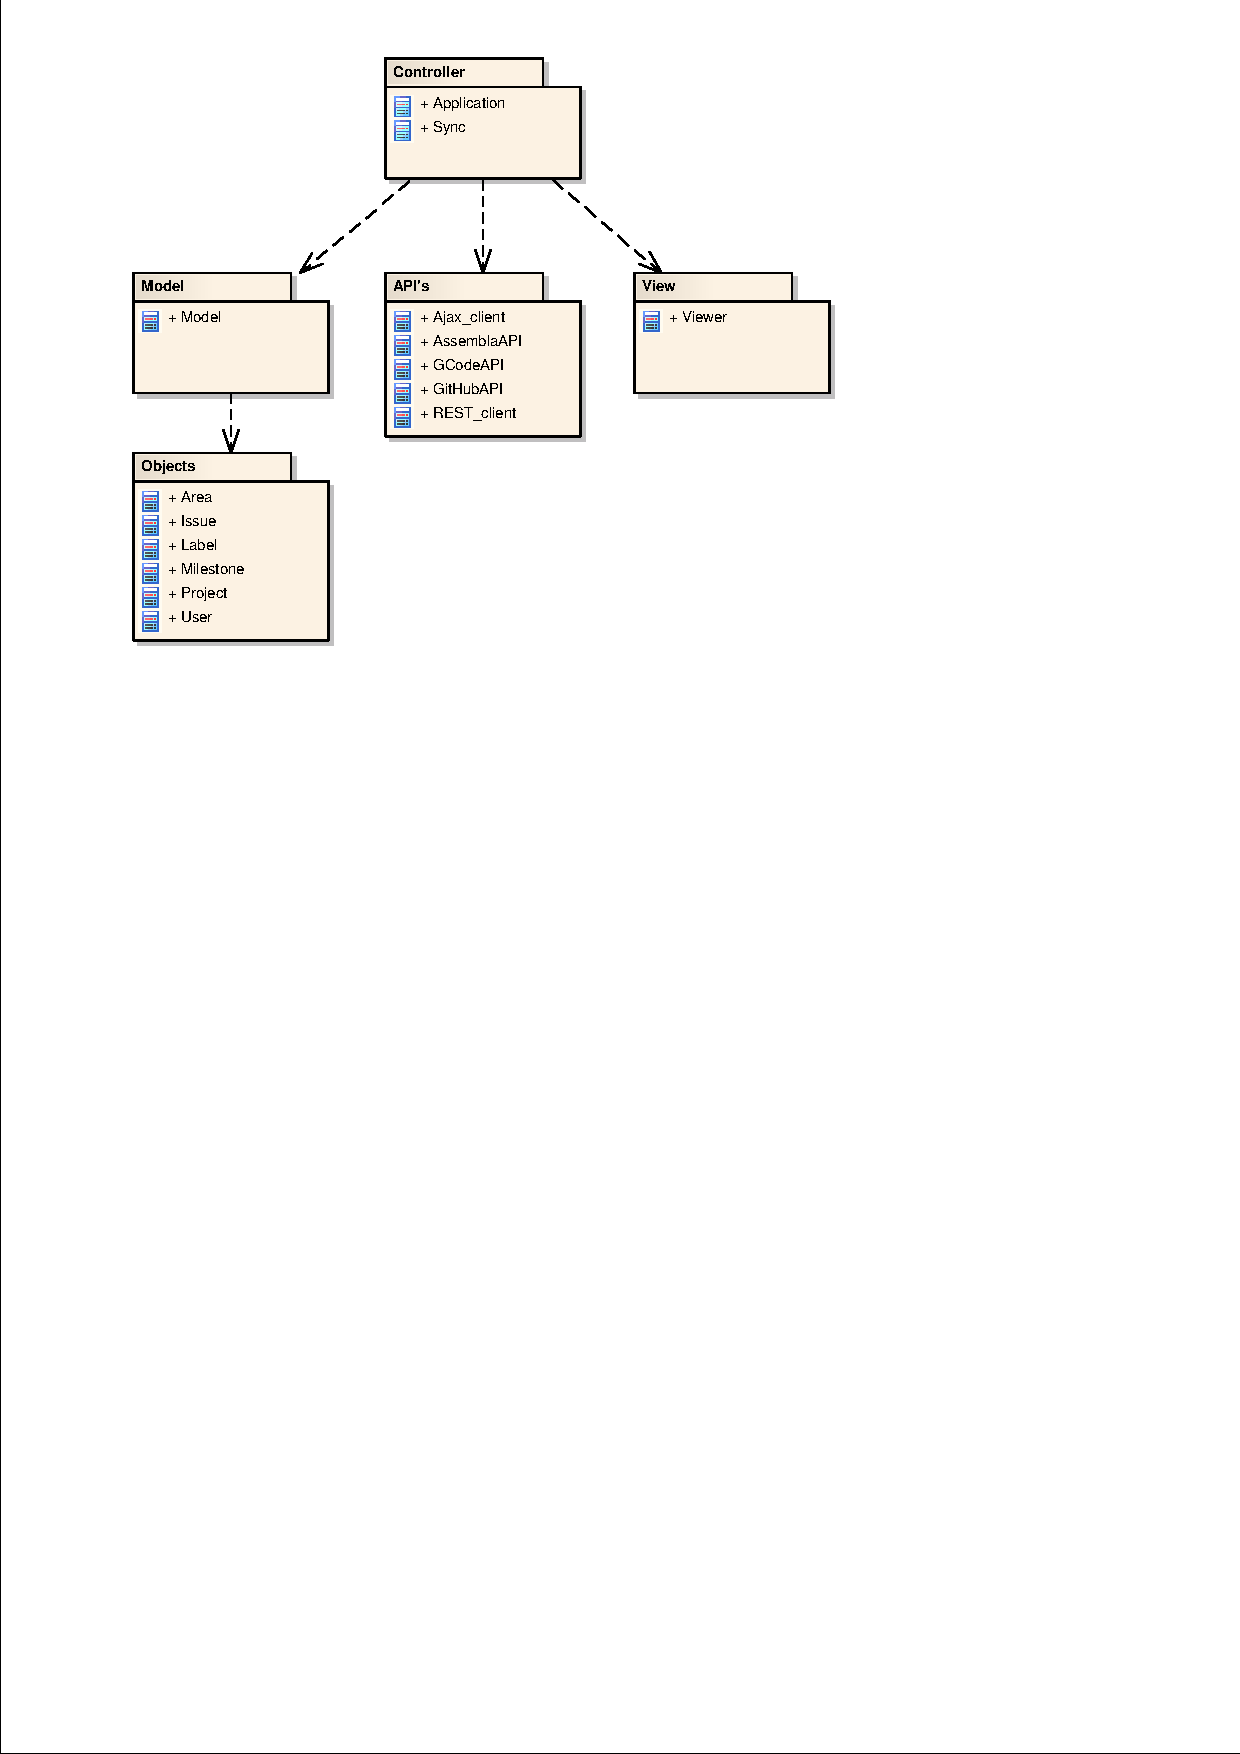
\includegraphics[width=11cm,scale=1,trim=20mm 185mm 60mm 10mm, clip]{figures/class-model}
	\caption{Rozdělení do balíčků}
	\label{fig:class-model}
\end{center}
\end{figure}

\subsection{Controller}

Balíček tříd, které se starají o samotný běh aplikace a synchronizaci se vzdálenými servery.

\subsubsection{Application}

Tato třída je využívána hlavně při startu aplikace. Má dva hlavní úkoly - načíst a naparsovat konfigurační soubor, který je uložený ve formátu JSON, a založit připojení k databázi.

\subsubsection{Sync}

Synchronizace mezi aplikací a vzdálenými servery má na starosti právě tato třída. Přijímá nové objekty z dialogů, předává je do modelové části a stará se o volání odpovídajících API (podle typu projektu). Žádná velká logika v ní není, stará se hlavně o předávání požadavků do jiných vrstev aplikace (model a view).

\subsection{Model}

Balíček tříd, které se starají o komunikaci s databází.

\subsubsection{Model}

V této třídě jsou umístěny všechny metody, které přímo komunikují s databází. Největší skupinou metod jsou ty, které poskytují CRUD (create, read, update, delete) nad všemi entitami zastoupenými v systému. Zároveň je zde několik metod, které usnadňují často používané operace, jako je načítání štítků ke konkrétnímu úkolu nebo zjištění procentuálního dokončení jednotlivých projektů.

\subsection{API's}

Balíček tříd, které jsou používány při komunikaci se vzdálenými servery. Třídy slouží ke zpřístupnění API vzdáleného serveru aplikaci.

\subsubsection{xxxAPI}

Třídy se sufixem \uv{API} jsou v systému celkem tři (AssemblaAPI, GCodeAPI a GitHubAPI). Každá odpovídá jednomu verzovacímu serveru, se kterým je systém synchronizovatelný. Všechny mají společného předka - abstraktní třídu API - a to z důvodu usnadnění budoucího rozšíření aplikace o další servery. Bohužel v JavaScriptu není implementace dědění úplně dokonalá, takže jde spíš o doporučení než povinnost. Třídy využívají každá svého klienta pro volání vzdálených serverů. U Assembly a Google Code je to REST\_client, GitHub používá Ajax\_client. Zároveň mají na starost naparsování entit do odpovídajícího formátu (JSON nebo XML), aby se dali předat klientovi, který je přepošle ven.

\subsubsection{Ajax\_client}

Tato třída je spolu s tou následující dalším usnadněním budoucího rozšiřování aplikace o spolupráci s dalšími servery. Slouží k odesílání požadavků v podobě AJAXových volání. V momentálním stavu aplikace ji využívá pouze API služby GitHub. Na vstup získává požadavek ve formátu JSON a odesílá ji na stanovenou URL adresu pomocí zvolené metody (POST, PUT, DELETE). Po přijetí odpovědi předá získaný výsledek zpět API do metody, jejíž jméno klient získal při úvodním volání.

\subsubsection{REST\_client}

Protože zbylé dva servery, tzn. Assembla a Google Code, fungují na architektuře označované jako REST (REpresentational State Transfer) bylo nutné vytvořit druhého klienta, který usnadní komunikaci s těmito servery. Požadavky jsou narozdíl od předchozí třídy ve formátu XML souboru. Zpracování odpovědi se příliš neliší od předchozí třídy. Jediný rozdíl tkví v naparsování odpovědi do objektu reprezentujícího XML dokument.

\subsection{View}

Balíček tříd, které mění vizuální stránku aplikace.

\subsubsection{Viewer}

V rámci dodržení architektury MVC došlo k oddělení vytváření vizuální stránky aplikace do samostatné třídy. Ta se stará o výpis seznamu úkolů, projektů a dalších grafických prvků. Grafická stránka aplikace je vytvářena na základě několika šablon, které jsou uloženy v samostatných souborech, aby bylo možné je v budoucnu snadno pozměnit bez ovlivnění funkčnosti aplikace. Takže například výpis úkolů je složen z x částí, kde každá část pochází z jedné šablony, která se opakuje.

\subsection{Entity}

Balíček tříd, které reprezentují jednotlivé entity v systému. Třídy byly již popsány v sekci Metodika - Doménový model.

\section{Bezpečnost}

U webových aplikací je kladen velký důraz na zabezpečení aplikace proti vnějšímu zásahu ať už za účelem získání soukromých informací nebo poškození aplikace. Vytvářená aplikace sice není přímo webová, ale i tak byla otázka zabezpečení důležitá. Nejzranitelnější částí aplikace je samotná komunikace se vzdálenými servery jednotlivých verzovacích systémů. Není totiž možné použít pokročilé zabezpečovací techniky jako je OAuth2 (používá Github) nebo AuthSub proxy (Google Code). V obou případech je totiž nutnou podmínkou fixní URL, na které klientská aplikace běží. Vytvářená aplikace běží přímo na uživatelově počítači a ne někde na vzdáleném serveru a jako taková nemá přidělenou globálně přístupnou URL. Jedinou možností zabezpečení aplikace tak zůstala Basic authentication, u které stačí připojit speciální hlavičku \uv{Authorization} přímo do odesílaného požadavku. Jejím obsahem je slovo \uv{Basic} a zahashované spojení uživatelského jména a hesla kódováním Base64. Tento hash lze snadno přeložit zpět na čitelnou formu, protože účelem toho algoritmu není šifrování přenášených dat ale pouze možnost zapsat binární data do tisknutelných znaků ASCII. Každý z trojice verzovacích systémů (Assembla, Github, Google Code) používá jiný způsob zabezpečení komunikace (tzn. autentizaci a autorizaci). 

\subsection{Zabezpečení serveru Assembla}

U tohoto serveru existuje jediný způsob zabezpečení\cite{assemblaauth} a sice použití Basic Authentication, které vlastně žádné zabezpečení neposkytuje, slouží pouze k autentizaci požadavku na API.

\subsection{Zabezpečení serveru GitHub}

V případě služby Github je situace komplikovanější\cite{github:summary}. Upřednostňovaná forma přihlášení k serveru je OAuth2\cite{github:oauth}, což je protokol sloužící externím aplikacím k požádání o autorizaci bez toho, aby získaly heslo uživatele. Je preferována před Basic Authentication protože umožňuje omezit přístup jen k určitým datům a uživatel může tento přístup kdykoliv zrušit. Postup získání tohoto povolení je jednoduchý. Vývojář nejdřív svou aplikace zaregistruje a tím získá dva údaje: unikátní ID klienta a tajné heslo, které by nemělo být nikde zveřejněno. Pomocí těchto dvou údajů se klientská aplikace autentifikuje u serveru a po vyplnění přihlašovacího jména a hesla je uživatel přesměrován zpět do klientské aplikace s náhodně vygenerovaným tokenem (buď přímo v URL, nebo v hlavičce odpovědi). Tento token je pak používán u každého požadavku na server až do ukončení session. Tento postup je ale pro aplikace běžící na desktopu nepoužitelný protože není kam uživatele přesměrovat. Proto Github zároveň podporuje i Basic Authentication.

\subsection{Zabezpečení serveru Google Code}

Google Code používá službu\cite{googleauth} založenou na podobném principu jako je OAuth2. Zde ale není nutná registrace aplikace přímo na serveru. Aplikace, která vyžaduje přístup k soukromým datům uživatele, a nemůže tedy využit anonymního přístupu, přesměruje uživatele na speciální URL, kde se vyplní uživatelské jméno a heslo a uživatel je posléze přesměrován zpět do klientské aplikace s vygenerovaným AuthSub tokenem uloženým v odpovědi. Obsahem požadavku jsou čtyři údaje:

\begin{enumerate}
\item next - URL, na kterou má být uživatel přesměrován (URL aplikace)
\item scope – určí, že je požadován vstup do Google Code
\item secure – určuje, zda klient požaduje zabezpečený token
\item session – určuje, zda může být token konvertován na multi-use (session) token
\end{enumerate}

Pro aplikace běžící na desktopu je ale nutné použít nižší úroveň zabezpečení – ClientLogin. Ten spočívá v odeslaní požadavku v daném formátu na určitou URL. V odpovědi, pokud je autentizace úspěšná, jsou navrácena tři alfanumerické kódy. Klientskou aplikaci ale zajímá pouze ten poslední, který je použit jako autorizační token při odesílání požadavku (podobně jako se u Basic authentication odesílá Base64 hash). Kamenem úrazu této metody je ale úvodní požadavek, ve kterém je odesláno uživatelské jméno a heslo v čitelné formě přímo v požadavku (konkrétně v POST), takže pokud by provoz na síti někdo odposlouchával, získá snadno přístup do účtu uživatele. Bohužel jiná forma autentizace pro desktopové aplikace neexistuje ani u jedné z těchto tří služeb.

\section{Titanium studio}

\subsection{Představení}

Samotné Titanium Studio je pouze vývojové prostředí, které usnadňuje práci s platformou Titanium. Tato není závislá na operačním systému. Je tak možné vytvářet aplikace zároveň pro Windows, Linux nebo Mac. Stejně tak pokud v budoucnu dojde k vytváření mobilní verzi dané aplikace, je možné některé části kódu znovupoužít a předělat jen grafickou stránku aplikace. Jádrem celé platformy je API\cite{titanium:api}, které je přístupné přes globální objekt Titanium. Přes něj se dají snadno vytvářet další okna aplikace, různá menu a poskytuje snadný přístup k souborům uloženým na filesystému nebo k tabulkám v databázi. Celé API je složené z mnoha modulů, které alespoň ve zkratce představím.

\begin{itemize}
\item Titanium - top-level modul sloužící jako kontejner pro všechny ostatní moduly
\item Titanium.API - přístup do jádra platformy Titanium
\item Titanium.Analytics - správa analytických událostí
\item Titanium.App - správa aktuálně běžící aplikace
\item Titanium.Codec - poskytuje možnost dekódování/zakódování multimédií
\item Titanium.Database - přístup do databáze
\item Titanium.Filesystem - přístup do filesystému
\item Titanium.JSON - umožňuje de/serializovat JSON pole
\item Titanium.Media - správa zvuku
\item Titanium.Network - správa síťových spojení
\item Titanium.Notification - možnost zobrazování notifikací na ploše počítače
\item Titanium.Platform - přístup k funkcím specifické platformy
\item Titanium.Process - možnost vytváření procesů
\item Titanium.UI - správa UI aplikace
\item Titanium.UpdateManager - správa verzování aplikace (instalace updatů)
\item Titanium.Worker - správa vláken Worker
\end{itemize}

\subsubsection{Databáze}

Jako databázový engine se používá SQLite\cite{sqlite}, kde je celá databáze uložena v jednom souboru a tím se snadno zálohuje nebo přenáší na jiný počítač. O připojení k databázi se postará globální objekt, stačí znát jméno databáze, které je možné předem určit. Po připojení se získá objekt, na kterém už lze pokládat dotazy na databázi v jazyce SQL. Jak může takové volání vypadat, ukazuje následující příklad:

\begin{quote}
DB.execute("INSERT INTO images (title, description) VALUES (?, ?)", "test", "description");
\end{quote}

V tomto příkladě je vidět obrana proti útoku SQL Injection, které je realizováno voláním metody s argumenty, které jsou následně escapovány.

\subsubsection{AJAX}

Další velmi důležitou součástí API je mechanismus pro asynchronní volání vzdálených serverů - AJAX. Provádění těchto volání má jednu velkou výhodu oproti tomu samému volání v prohlížeči – není zde problém s cross-domain policy\cite{sameorigin}, což je v zásadě ochrana proti vykonávání JavaScriptu na jiném serveru, kterou mají prohlížeče zabudovánu v sobě. 

Během volání je možné sledovat odpovědi serveru a je možné definovat si funkce, které na tyto události zareagují. API poskytuje plnou kontrolu nad tím jaká data se na server posílají a jaká metoda v rámci protokolu HTTP se použije. API verzovacích serverů totiž rozlišují požadavky i podle této metody. Takže pokud má volání něco na serveru smazat, je třeba použít metodu DELETE. Pokud je naopak účelem něco založit (úkol, projekt, milník), použije se metoda PUT. K běžnému stahování obsahu - čtení - postačí metoda GET příp. POST.

Protože API služeb Assembla a Google Code běží na architektuře REST, je nutné mít možnost posílat voláním i soubory, konkrétně ve formátu XML. Tento požadavek byl poměrně problematický, protože v dokumentaci API není toto dostatečně popsáno. Naštěstí jsou na internetu různé tutoriály, které pomohou a navedou člověka správným směrem. Samotné sestavování AJAXového volání je hodně low-level a člověk musí řešit spousty technických věcí. Například u zmiňovaného posílání souborů je nutné ručně sestavit hlavičku požadavku, aby došel ve správném tvaru na server. Server Assembla například soubor nepřijme, pokud ve volání nepřijde hlavička:

\begin{quote}
Accept : application\slash xml
\end{quote}

\subsubsection{Vytváření oken a nabídek}

Každá aplikace na desktopu sestává z více částí. Hlavní viditelnou částí je samotné okno aplikace. V prostředí Titanium Studia je možné definovat jak toto okno bude velké, zda bude maximalizované a jak s ním bude moct uživatel manipulovat. Všechny tyto volby jsou uloženy v XML souboru, takže se dají snadno upravovat.

Pokud je potřeba za běhu aplikace vytvořit nové okno, umožní to zmiňované API. Nastaví se jeho velikost, poloha, obsah (obvykle HTML soubor) a další volby. Titanium ho pak vykreslí a pak s ním lze dále pracovat. Všechny Javascriptové soubory, které se budou v novém okně používat, jen nutné vložit do toho HTML souboru. A to i když jsou již vloženy do hlavního okna aplikace. Jediné, co se vloží automaticky, je globální objekt Titanium, který zpřístupňuje API.

Většina aplikací na desktopu mívá hlavní menu v šedém pruhu hned na vrchu okna aplikace. I v rámci Titanium Studia je možné toto menu vytvořit. Funguje to jednoduše. Na API stačí zavolat metodu Titanium.UI.createMenu, která vytvoří objekt, reprezentující celé menu. Do něj pak lze buď přidávat další podmenu nebo přímo jednotlivé položky. Menu funguje na principu událostí, takže pokud uživatel na některou z položek klikne, dojde k zavolání metody definované při zakládání dané položky.

\subsection{Výhody a nevýhody}

Mezi hlavní výhody využívání Titanium API rozhodně patří:

\begin{itemize}
\item snadná práce s databází
\item možnost posílat AJAXová volání na vzdálené servery bez omezení
\item snadná práce s UI aplikace (vytváření dalších oken a nabídek)
\end{itemize}

Tyto výhody určitě převyšují dále zmíněné nevýhody, které vyplývají z používání Titanium Studia.

\begin{itemize}
\item debuggování
\item málo chybových hlášení
\end{itemize}

Velkou nevýhodou je rozhodně debugování (nalézání a oprava chyb) aplikace. V rámci běhu aplikace existuje sice možnost sledovat výpis hlášení v okně konzole, ale mnohé chyby se zde neobjeví a aplikace prostě zamrzne. Vývoj se tak občas dost zpomaluje, protože hloupé chyby se hledají obtížně a jeden malý překlep může způsobit velké problémy.

\subsection{Využití API v aplikaci}

Vytvořená aplikace je pevně spojená s Titanium API a nemůže bez něj prakticky existovat. Mezi nejdůležitější využívané funkce patří rozhodně přístup k databázi a filesystému. To jsou funkce, které by byly bez API poměrně obtížně realizovatelné. Je toho ale mnohem víc. Vzhledem k tomu, že jedním z poslání aplikace je synchronizace se vzdálenými servery, je hojně využívána i část síťová, tzn. AJAXová volání. 

Protože JavaScript není úplně objektový jazyk a některé konstrukce nejsou možné, pomohlo Titanium API i zde. Jde například o globální předávání objektů, aby nebylo potřeba je pokaždé vytvářet znovu, což by bylo velké plýtvání prostředky a nejspíš by to výrazně zpomalilo celou aplikaci. Objekty se proto po vytvoření uloží do globální úložiště (ač je to v rozporu s principy objektového programování), které je plně v režii Titanium API a odkud je možné si je kdykoliv vyžádat a vykonávat na nich operace. Takto je například uložené spojení s databází nebo objekt starající se o synchronizaci se vzdálenými servery.

Jak je API v aplikace využíváno, bude nejlépe patrné z nějakého příkladu. Následující model demonstruje workflow přidání nového úkolu do projektu, který je svázán s repozitářem na serveru GitHub. Rámcově lze workflow vyjádřit i textově:

\begin{enumerate}
\item uživatel iniciuje obsluhu události
\item od uživatele se získá nějaký vstup
\item uložení vstupu do databáze
\item zavolání vzdáleného serveru
\item zpracování odpovědi od serveru
\end{enumerate}

\begin{figure}[h]
\begin{center}
	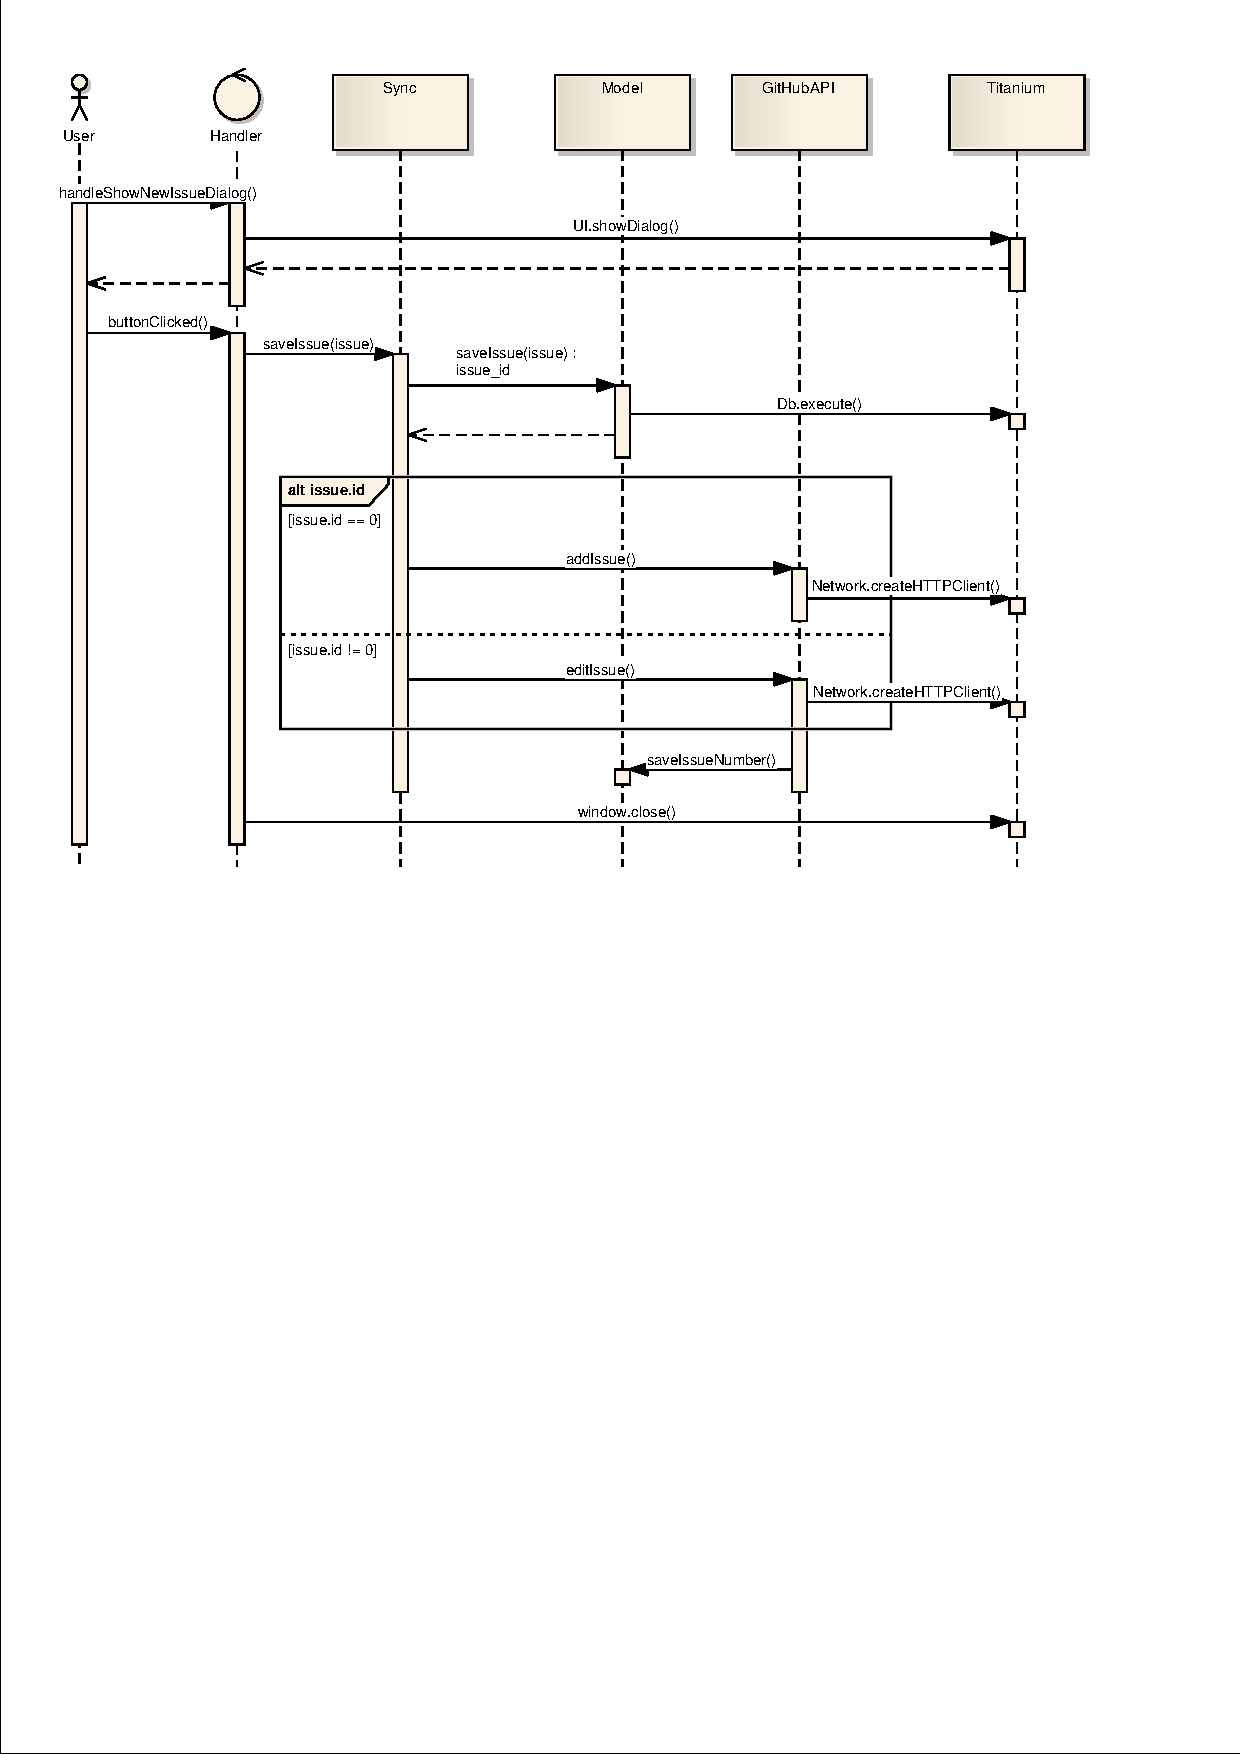
\includegraphics[width=15cm,scale=2,trim=10mm 145mm 10mm 10mm, clip]{figures/vyuziti-api}
	\caption{Využití API v aplikaci}
	\label{fig:vyuziti-api}
\end{center}
\end{figure}

Jak je vidět z diagramu \ref{fig:vyuziti-api}, API je skutečně integrální součástí aplikace a poskytuje spousty důležitých funkcí, které hodně zrychlují a usnadňují vývoj celé aplikace.

%*****************************************************************************
%*****************************************************************************
%*****************************************************************************

\chapter{Nasazení aplikace}

Titanium framework je deklarován jako multiplatformní a neměl by tedy být problém s přenosem vytvořené aplikace na jiný operační systém. Bohužel dle získané zkušenosti tomu tak není. Aplikace byla primárně vyvíjena na operačním systému Windows 7, kde se neobjevily žádné větší problémy. Ty ale nastaly při pokusu o spuštění na jiné platformě. Pokus o nasazení byl proveden na dalších dvou různých operačních systémech. Šlo o operační systém Debian\cite{debian}, jakožto zástupce Linuxu, a Mac OS X\cite{mac}. Ani na jednom ze zmiňovaných systémů se nepodařilo aplikaci plně zprovoznit.

Další problémy se objevily ve finální fázi, kdy měla být aplikace připravena pro instalaci na jiných počítačích. Titanium Studio totiž umí aplikaci přeložit pouze pro platformu, na~které momentálně běží. Takže například není možné na Windows přeložit aplikaci určenou pro Mac a obráceně. A to navzdory tomu, že překlad je prováděn za asistence vzdáleného serveru, což mimochodem proces překladu výrazně zpomaluje. O multiplatformnosti Titanium Studia lze tedy oprávněně pochybovat.

\section{Linux}
Test nasazení byl proveden na virtuálním stroji s nainstalovaným operačním systémem Debian ve verzi 6.0.3 (i386).

Zde se ukázalo jako nemožné samotné spuštění vývojového prostředí Titanium Studio, ve kterém se aplikace kompiluje. Možnou příčinou je fakt, že aplikace je distribuována v~archivu typu zip, který není primárně určen pro Linux a nezachovává symbolické odkazy. Veškeré pokusy o nápravu skončily neúspěchem. Podle oficiálního fóra má tyto problémy více uživatelů.

\section{Mac OS X}

Testování na této platformě bylo poměrně problematické, protože odpovídající operační systém nebyl k dispozici. Pokusy o nasazení byly prováděny pouze na soukromém počítači vedoucího této práce a lze říci, že nebyly 100\% úspěšné. Na rozdíl od Linuxu sice bylo možné nainstalovat a spustit vývojové prostředí, ale se samotnou aplikací už ne. Ani po mnoha pokusech se ji nezdařilo plně zprovoznit. Neustále se objevovaly chyby na úrovni OS, které byly obtížně odstranitelné.

%*****************************************************************************
%*****************************************************************************
%*****************************************************************************

\chapter{Testování}

Každý správný vývojový cyklus software obsahuje fázi testování\cite{zivotnicyklus}. Aplikaci lze testovat ve více vlnách, kdy se pokaždé provádí jiný typ testů. Obecně lze testy rozdělit do těchto dvou hlavních skupin - blackbox a whitebox.

Blackbox testy testují aplikaci zvenku a nepotřebují vědět, co se děje uvnitř. Proto se testy označují jako \uv{blackbox}. U těchto testů je aplikace černou skříňkou a jsou k dispozici pouze dva otvory - vstup a výstup. Do aplikace se pošle nějaký vstup a očekává se určitý výstup. Pokud výstup splňuje očekávání, test byl úspěšný. Hlavní výhodou těchto testů je jejich jednoduchost, protože není potřeba znát konkrétní obsah tříd a metod uvnitř aplikace. Do blackbox testů lze zařadit testy rozhraní (Selenium \cite{selenium}), akceptační nebo zátěžové.

Naproti tomu whitebox testy vyžadují znalost kódu aplikace a jsou pevněji svázány s implementací uvnitř. Tyto testy jsou mnohem konkrétnější a obvykle testují menší celky aplikace (balíčky -$>$ třídy -$>$ metody). Postup testování může být dvojí. Buď se testují nejdřív největší celky a postupně se zanořuje, nebo se naopak postupuje od nejmenších jednotek po ty největší. Těmto testům se říká jednotkové (angl. unit testy). Do kategorie whitebox testů spadají také integrační testy, které ověřují, zda spolu jednotlivé komponenty aplikace komunikují tak, jak mají.

\section{Použitý způsob testování}

Testování této aplikace není tak snadné jako u webových aplikací. Některé testy nejsou realizovatelné (např. testy rozhraní pomocí nástroje Selenium), protože aplikace není spustitelná v prohlížeči. Toto omezení způsobuje globální objekt Titanium, který není v prostředí prohlížeče k dispozici a aplikace se tak stává nepoužitelnou.

Pro testování je využita JavaScriptová knihovna jsUnity\cite{jsunity}, pomocí které jdou poměrně snadno vytvářet jednotkové testy. Poskytuje jednak běhové prostředí a hlavně assertovací metody, které ověří výsledek testu. Knihovnu je potřeba trochu poupravit, aby výsledek testů vypsala do okna a do výstupu, kde by se výsledek ztratil v záplavě runtime hlášení.

Testy jsou seskupeny v objektech, které se spouští metodou \emph{jsUnity.run()}. Aby nebyly při každém testu znovu zakládány všechny objekty, vytvoří se předem a během testů už se na nich pouze volají metody. Korektní postup je sice jejich zakládání před každým testem v metodě \emph{setUp()}, ale tento způsob se ukázal jako hodně pomalý a bylo od něj upuštěno. Nejpomalejší operace je určitě založení spojení s databází, která je potřeba u většiny testů a protože testy mají být hlavně rychlé, bylo nutné zvolit nějaký kompromis.

\section{Testování asynchronních volání}

V aplikaci se mnoho operací děje asynchronně, aby aplikace nezamrzala (hlavně při spojení se vzdálenými servery). Tento způsob běhu aplikace bohužel znemožňuje testování jednotkovými testy. Jak vypadá asynchronní volání ukazuje diagram \ref{fig:async-tests}.

\begin{figure}[h]
\begin{center}
	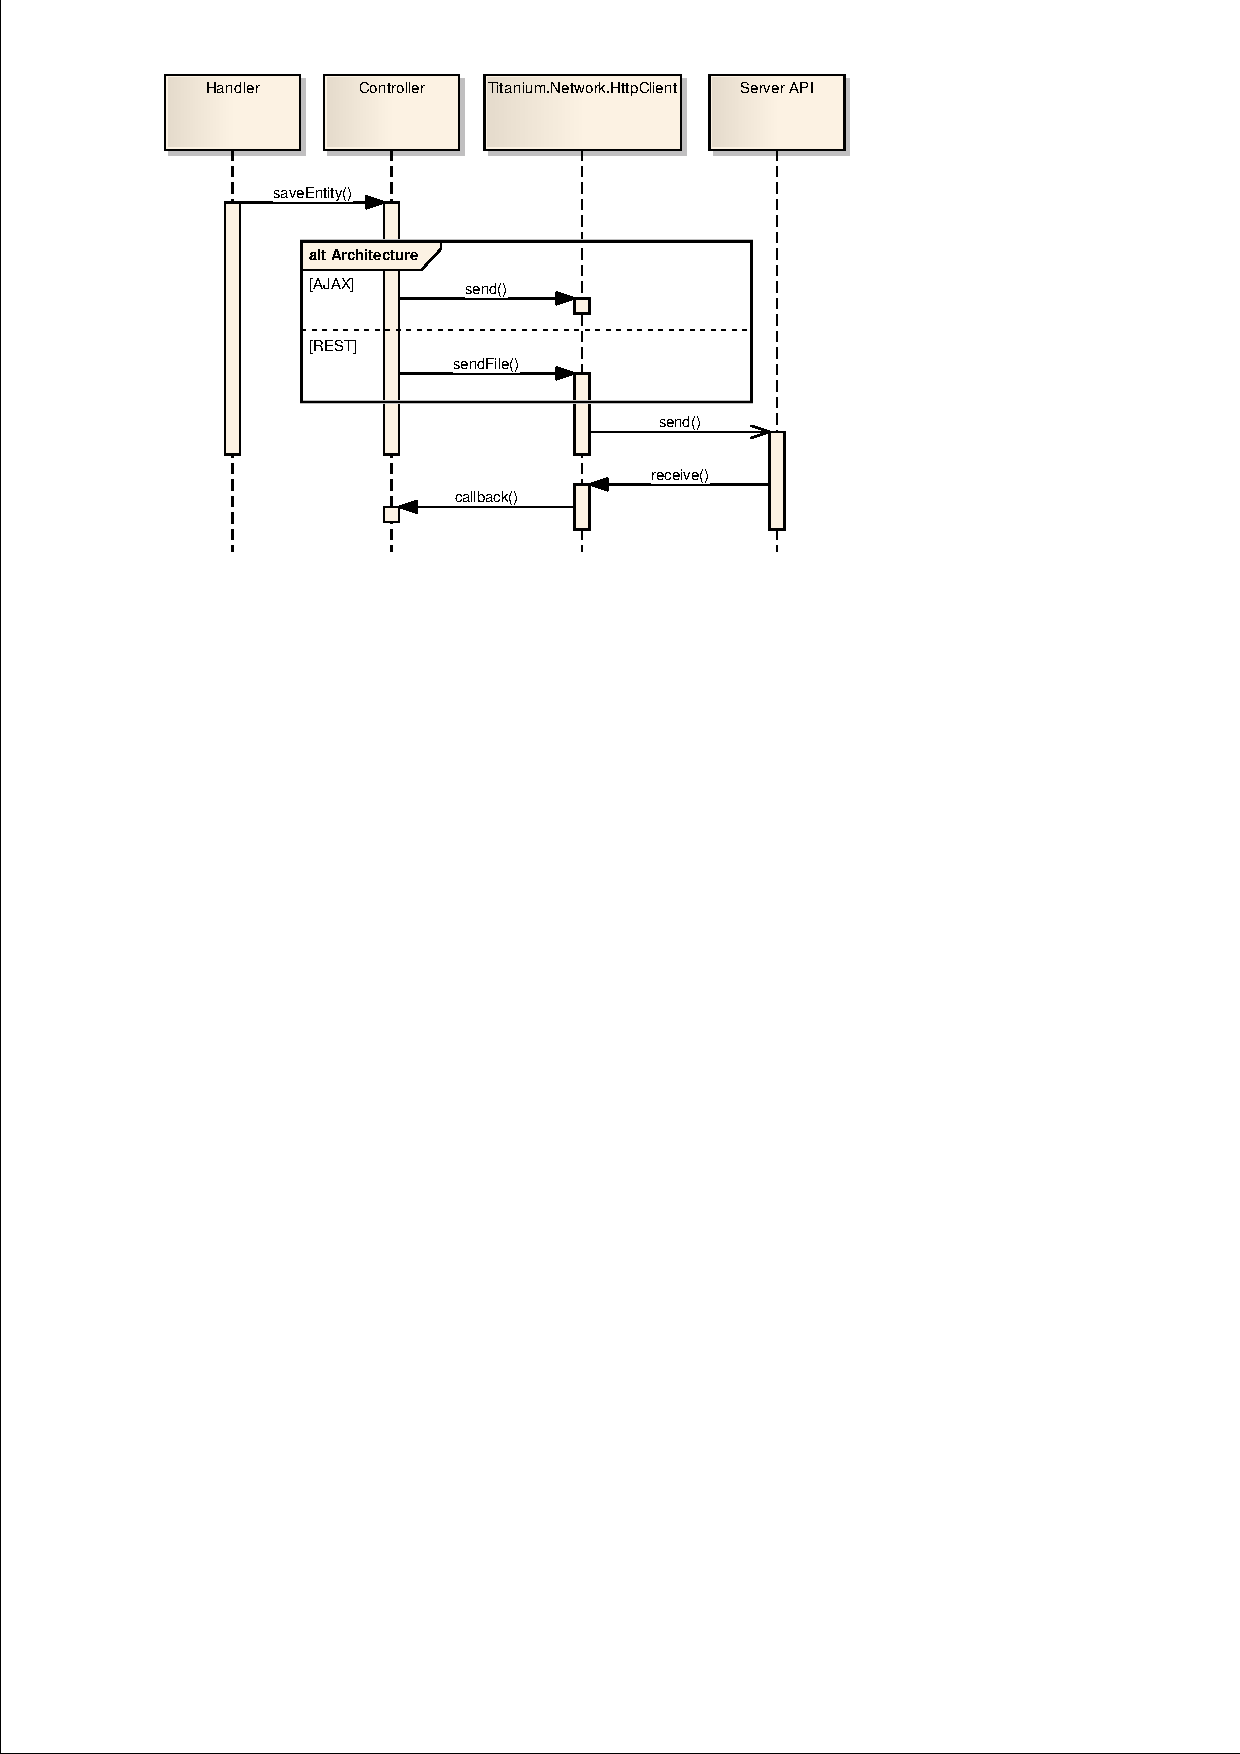
\includegraphics[width=15cm,trim=10mm 205mm 40mm 10mm, clip]{figures/async-tests}
	\caption{Asynchronní volání}
	\label{fig:async-tests}
\end{center}
\end{figure}

Problém, který zabraňuje testování, vzniká v kroku č.3 - předání callbacku. Během testování se o volání metod stará běhové prostředí a není možné volat jednotlivé metody (testy) samostatně. Důsledkem tohoto chování je nemožnost \uv{vrátit} se z HTTP klienta zpět do testu a vyhodnotit správnost odpovědi.

\section{Zátěžové testy}

Součástí fáze testování této práce jsou také zátěžové testy, jejichž úkolem je ověřit, jak rychle některé operace probíhají. Jako operace byla zvolena ta, která je využívána nejčastěji, a sice výpis úkolů z daného projektu. Při používání aplikace se totiž ukázalo, že tato akce trvá poměrně dlouho a zátěžové testy by mohly ukázat, jak moc závažný problém to je.

Zátěžové testy jsou postaveny na podobném principu jako jednotkové testy až na to, že zde se nesleduje výsledek testu, ale pouze jeho průběh. Test probíhá ve více iteracích, aby byla zátěž vystupňována. Bylo vytvořeno celkem 7 scénářů, které byly postupně otestovány:

\begin{itemize}
\item prázdný úkol (bez štítků a přiřazení)
\item úkol s jedním štítkem
\item úkol se dvěma štítky
\item úkol přiřazený uživateli s jedním štítkem
\item úkol přiřazený uživateli se dvěma štítky
\item úkol přiřazený uživateli s pěti štítky
\item úkol přiřazený uživateli s deseti štítky
\end{itemize}

Součástí každé iterace je vložení dalšího úkolu (příp. se štítky a uživatelem) do databáze a zavolání metody, starající se o načítání úkolů z databáze. Tím postupně narůstá zátěž, protože počet úkolů v databázi roste. Iterací bylo při každém testu celkem padesát. Čas spotřebovaný v rámci jedné iterace je měřen pomocí objektu Date a jeho metody getTime(). Tento čas je posléze vypsán na výstup a je dále ručně zpracováván. Hrubá data z těchto testů jsou k nalezení v přílohách této práce. Z těchto změřených dat byl také pro lepší názornost vytvořen graf, který je vložen níže. Jeho průběh není úplně hladký, což způsobuje pravděpodobně fakt, že testovací prostředí není úplně izolované od dalších procesů běžících na stejném počítači a procesor tak může dát prioritu jiné aplikaci a test se zpomalí. Dalším důvodem může být to, že je nutné číst data z pevného disku (databáze), což může ve stejnou chvíli chtít víc aplikací. Aplikace se tedy chová dle očekávání, protože graf zátěže stoupá lineárně. V grafu nelze pozorovat ani žádné extrémní výkyvy, které by ukazovaly na nějaké závažnější problémy.

\begin{figure}[h]
\begin{center}
	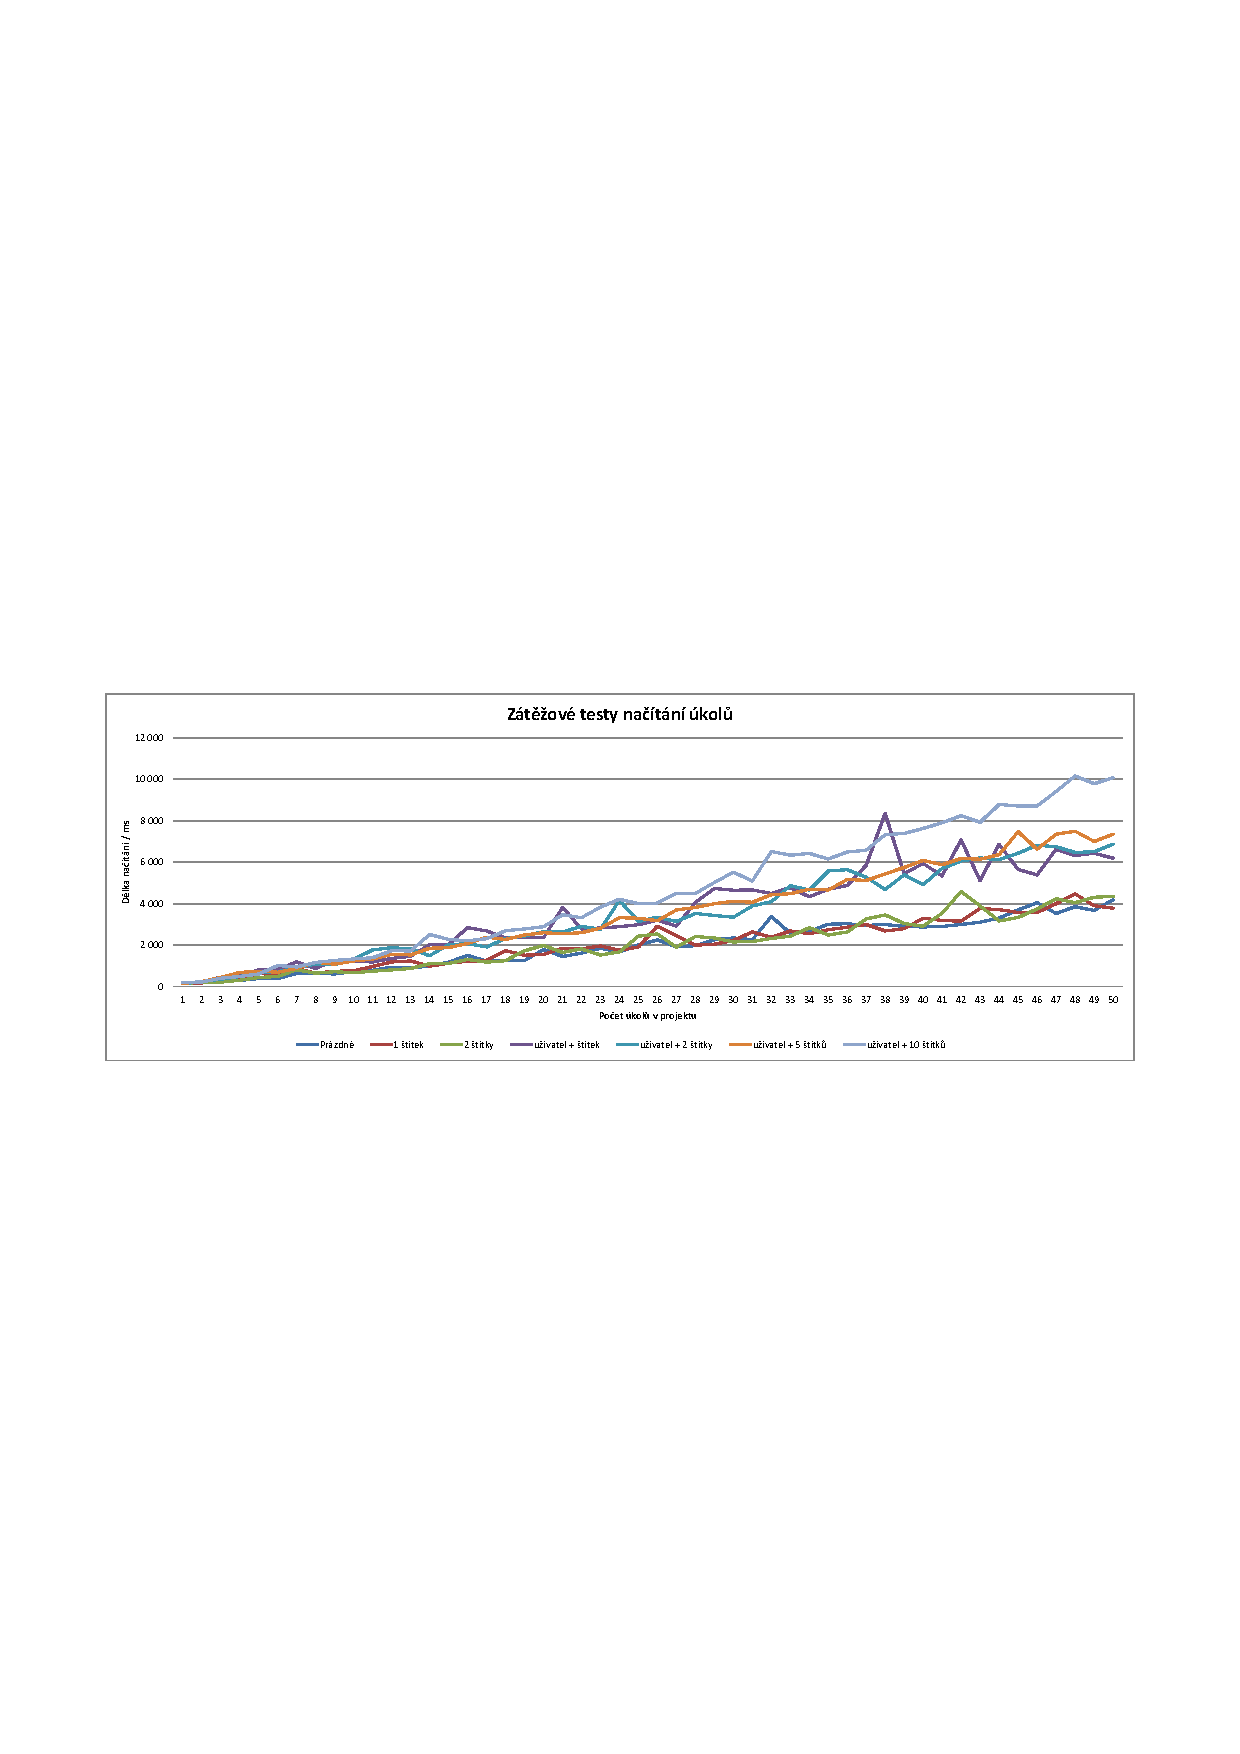
\includegraphics[trim=15mm 115mm 15mm 110mm, clip, width=15cm]{figures/zatezove-testy}
	\caption{Zátěžové testy}
	\label{fig:load-tests}
\end{center}
\end{figure}

%*****************************************************************************
%*****************************************************************************
%*****************************************************************************

\chapter{Shrnutí}

\section{Závěrečné zhodnocení aplikace}

Zhodnocení aplikace z pohledu splnění požadavků vychází ze srovnání user stories v části týkající se metodiky a nesplněných user stories uvedených v kapitole 6 - testování \ref{tab:failed-accept-tests}. Celkový počet user stories je 29, z toho 4 nebyly naplněny. Procentuální splnění požadavků se tak dostane na 86\%.

\section{Doporučení do dalšího vývoje}

Zátěžové testy ukázaly, že aplikace se stává poměrně pomalou s přibývajícími úkoly v jednotlivých projektech. Problém tkví ve čtení dat z databáze. Řešením by mohla být nějaká vyrovnávací paměť (cache), která by byla umístěna mezi databází a zbytkem aplikace. To s~sebou nutně přinese mnoho dalších komplikací a zrychlení aplikace tak může být poměrně drahé. Mezi největší problémy patří určitě volba úložiště vyrovnávací paměti a také její invalidace (smazání neaktuálních dat). Úložiště musí být dostatečně rychle přístupné, aby vůbec mělo smysl vyrovnávací paměť implementovat. Nasnadě je využití souborové cache, ale čtení dat z filesystému nemusí být zrovna nejrychlejší. Lepší by bylo ukládání dat do operační paměti, jenže k té nemá JavaScript přístup. Dalším problémem je invalidace cache, tedy odstranění neaktuálních dat z paměti. Je totiž poměrně velký problém určit, kdy už data nejsou aktuální.

Další funkce, na které se přišlo během vývoje a které byly zařazeny do kategorie \uv{hezké mít} (angl. nice-to-have) jsou tyto:

\begin{itemize}
\item sledování i cizích projektů
\item vytváření vlastních přehledů úkolů (kombinace štítků a projektů)
\item automatické sledování commitů do synchronizovaného repozitáře
\item modulárnější vizuální stránka s využitím knihovny MustacheJS\cite{mustache}
\end{itemize}

Tyto funkce se ukázaly buď jako obtížně realizovatelné (vyrovnávací paměť, vytváření vlastních přehledů) nebo poměrně zbytečné (MustacheJS, sledování commitů), ale přesto byly uloženy, aby se na ně nezapomnělo.

\subsection{Práce s IDE Titanium Studio}

Součástí zadání této práce byla i rešerše Titanium Studia. Jejím cílem bylo ověřit možnost použití této platformy k vývoji desktopových aplikací. Jedna strana jsou oficiální dokumentace a druhá její reálné používání, jak se ukázalo mnohokrát během vývoje. Ve fázi testování se ale ukázalo, že spoustě problémů se lze vyhnout tím, že se vývoj provádí v operačním systému Windows a ne na Linuxu nebo Macu, kde už jen samotné zprovoznění IDE se ukázalo jako problém.

Nicméně Titanium API poskytuje spousty funkcí, které by se jinak musely doprogramovávat ručně. Není tak nutné zahrnovat do aplikace skripty napsané v jiném jazyce (Titanium Studio podporuje vývoj v PHP, Ruby a Pythonu), ale je možné využít připravené rozhraní. Těžko si například představit, jak náročné by bylo vytvoření spojení s databází jen pomocí JavaScriptu.

Existuje však jeden velmi výrazný nedostatek - vychytávání chyb (debugging). To je v~tomto IDE velmi špatně zpracované. Autoři Titanium Studia sice nabízí rozšířený editor, který by měl mít debugging zpracovaný lépe, ale ten už není poskytováno zdarma, a to ani ke studijním účelům. Ve většině případů je tak vývojář na metodu pokus-omyl, kdy i oprava banálního překlepu může trvat velmi dlouho. Během vývoje této aplikace sice došlo k několika aktualizacím a IDE tak hlásí aspoň některé chyby, ale ve spoustě případů prostě jen zamrzne a neposkytne vůbec žádnou zpětnou vazbu o tom, co a kde se vlastně stalo.

Na základě získaných zkušeností lze Titanium Studio doporučit dalším vývojářům, kteří by chtěli vyvíjet desktopové aplikace v jiném jazyce než v Javě nebo C\#. V nejčtenějším IT magazínu v ČR Programuje.com jsem publikoval článek\cite{selfpromo}, představující Titanium Studio a práci s ním. Dle reakcí čtenářů lze usoudit, že platforma má před sebou budoucnost a má smysl ji dále rozvíjet.

\subsection{Psaní aplikace zcela v JavaScriptu}

Další teorií, kterou měla tato aplikace za cíl potvrdit nebo vyvrátit, byla otázka, zda je možné vytvořit aplikaci zcela v JavaScriptu bez pomoci dalších programovacích jazyků. Ukázalo se, že tento postup je možný, ale zahrnuje dost problémů a kompromisů. Není například možné vytvářet rozhraní (interface) ve smyslu Javy nebo i PHP. To samé se týká abstraktních tříd. Rozšiřování aplikace o další moduly tudíž není tak snadné, jak by mohlo teoreticky být.

Dalším problémem je to, že JavaScript není primárně objektový jazyk, ale spíš procedurální, a některé konstrukce se vytváří hodně neohrabaně. Problém, který se často objevoval, je ztráta kontextu objektu. Nebylo tak možné přímo volat metody objektu, i když se zrovna prováděl kód v jiné z jeho metod. Toto se stávalo hlavně při obsluze asynchronního volání, kdy si metoda musela získat svého vlastníka z globálního kontejneru, kam byly všechny velké třídy (Application, Sync, Viewer a Model) ukládány.

Neduhem aplikací napsaných v JavaScriptu je také příliš mnoho funkcí, které je nutné zakládat velmi často, a celý kód se tak znepřehledňuje kvůli velkému množství závorek. Tento problém by částečně mohla vyřešit knihovna CoffeeScript\cite{coffeescript}, která používá hlavně odsazování a spousty závorek nepotřebuje, protože je schopná si je \uv{domyslet}. Bohužel je určena hlavně pro Linux a její zprovoznění na Windows se ukázalo jako velmi problematické. Také by to znamenalo nutnost učit se novou syntaxi.

\chapter{Závěr}

Výsledkem této práce je nástroj, který v sobě integruje správu tří verzovacích serverů. Protože se poskytovaná API hodně liší, byla nutná spousta kompromisů pro zachování konzistence ovládání aplikace. Tím je sice uživatel ochuzen o několik extra funkcí poskytovaných těmito servery, ale to hlavní je v aplikaci umožněno. Tato práce nekladla důraz na vizuální stránku, která dost často rozhoduje o úspěchu aplikace.

Důležitou součástí vývoje software je testování ve všech různých podobách. Při vývoji tohoto nástroje to nebylo jinak. Během vývoje byly prováděny jednotkové (unit) testy, po dokončení implementační fáze bylo provedeno zátěžové testování výpisu úkolů, což se ukázalo jako časově velmi náročná operace. Úplně nakonec byly provedeny akceptační testy na~základě sepsaných user stories. Všechny provedené testy potvrdily funkčnost aplikace a jako taková je připravená k používání reálnými uživateli.

%*****************************************************************************
% Seznam literatury je v samostatnem souboru reference.bib. Ten
% upravte dle vlastnich potreb, potom zpracujte (a do textu
% zapracujte) pomoci prikazu bibtex a nasledne pdflatex (nebo
% latex). Druhy z nich alespon 2x, aby se poresily odkazy.

\bibliographystyle{csplainnat}
\bibliography{reference}

%*****************************************************************************
%*****************************************************************************
\chapter{Seznam použitých zkratek}

\begin{description}
\item[IDE] Integrated Development Environment
\item[GTD] Getting Things Done
\item[API] Application Programming Interface
\item[JSON] JavaScript Object Notation
\item[REST] Representational State Transfer
\item[HTML] HyperText Markup Language
\item[RUP] Rational Unified Process
\item[UML] Unified Modeling Language
\end{description}

%*****************************************************************************
\chapter{Instalační a uživatelská příručka}
\textbf{\large Tato příloha velmi žádoucí zejména u softwarových implementačních prací.}

%*****************************************************************************
\chapter{Obsah přiloženého CD}
\textbf{\large Tato příloha je povinná pro každou práci. Každá práce musí totiž obsahovat přiložené CD. Viz dále.}

Může vypadat například takto. Váš seznam samozřejmě bude odpovídat typu vaší práce. (viz \cite{infodp}):

\begin{figure}[h]
\begin{center}
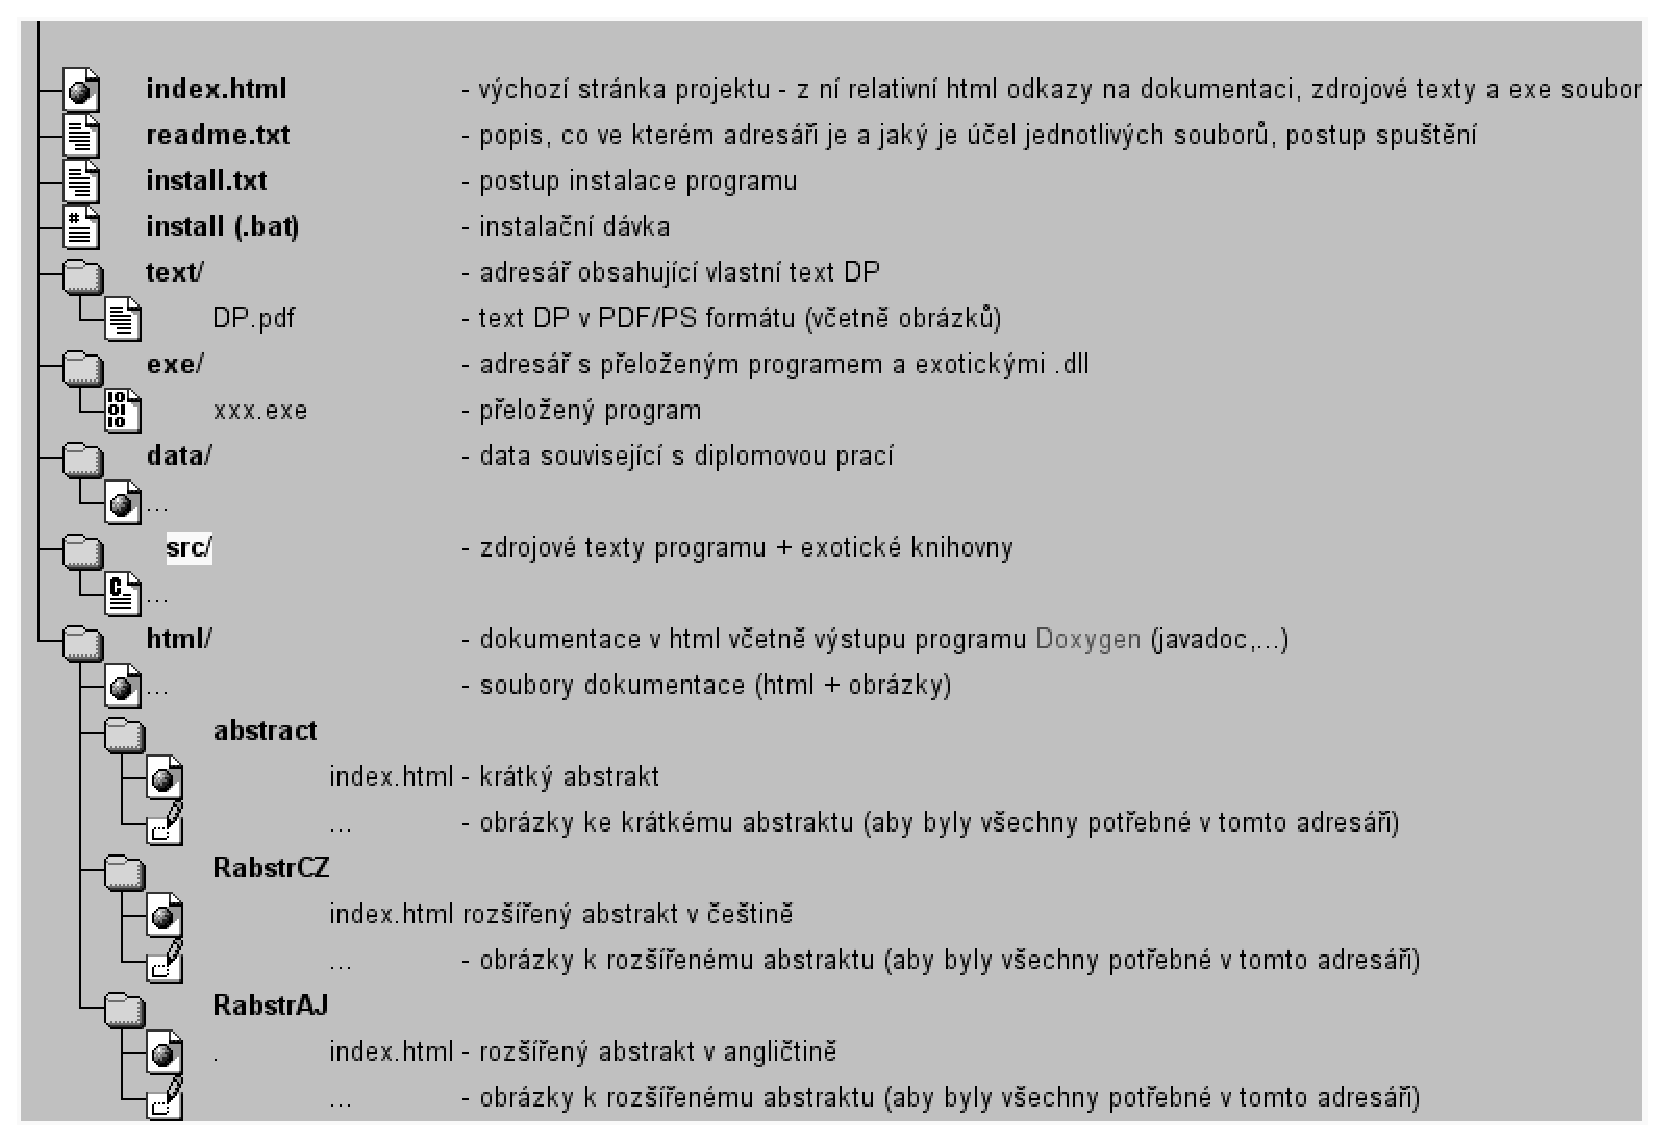
\includegraphics[width=14cm]{figures/seznamcd}
\caption{Seznam přiloženého CD --- příklad}
\label{fig:seznamcd}
\end{center}
\end{figure}

\end{document}